\chapter*{Cadre général du projet}
\addcontentsline{toc}{chapter}{Cadre général du projet}
\markboth{Cadre général du projet}{Cadre général du projet}
\label{chap:cadreGeneral}
%\minitoc

\section{Introduction}
Dans ce chapitre, nous nous intéresserons à l'introduction du cadre global du projet et à la description des exigences. Il s'agit en fait d'une introduction de l'organisme d'accueil, suivie d'une motivation et de la présentation du projet. Ensuite, nous présentons l'étude de l'existant et la solution proposée.

\section{Présentation de la société d'accueil}
Acteur indépendant et à dimension internationale, NeoLedge est une société française en forte croissance, qui s'appuie sur un réseau de partenaires privilégiés en Europe, en Amérique du Nord et en Afrique. Éditeur spécialisé dans la gestion électronique de documents, NeoLedge compte à son actif des centaines de clients, des dizaines de milliers d'utilisateurs quotidiens et des millions de documents gérés par ses solutions, dans le secteur public comme dans le secteur privé.

\medskip

Partenaire certifié Gold de Microsoft en ce qui concerne le développement d'applications et les plateformes cloud, NeoLedge accompagne des organisations 
pendant leur transition numérique.
NeoLedge s'appuie depuis ses débuts sur les techniques développées par Microsoft. 

\begin{figure}[h]
\centering
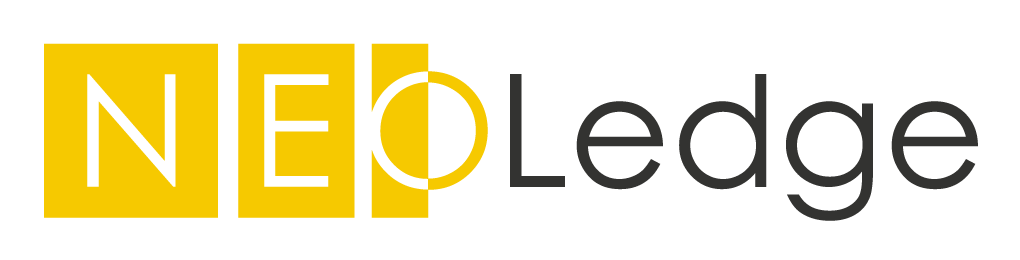
\includegraphics[width=0.5\textwidth]{neoledge_big_logo.png}
\caption{Logo de NeoLedge}
\label{fig:logoNeoledge}
\end{figure}

\subsection{Historique}

Archimed est un éditeur de logiciels français, créé en 1993 par trois fondateurs (Mongi Zidi, Olivier Walbecq et Eric Ruyffelaere) et dont le siège social est établi à Lille.
\medskip

Archimed est un éditeur indépendant spécialisé dans les logiciels de gestion documentaire depuis près de 25 ans. Elle a étendu son activité ECM ces dernières années à travers l'Afrique, l'Europe et l'Amérique du Nord.

\medskip
Afin d'accompagner son développement à l'international, la société a lancé NeoLedge, une nouvelle marque exclusivement dédiée à ses solutions et activités ECM. Le nom NeoLedge a été inspiré par les " new knowledge " - une nouvelle façon de gérer le contenu, d'optimiser le temps et de gagner en productivité.
